\subsection{Préparer l'échantillon}
\begin{center} $\ast\ast\ast$ Local F-6451 $\ast\ast\ast$ \end{center}
\begin{enumerate}
    \item Tiroir du haut: sortir le contenant en plastique identifié \textit{Stock imagerie Lightsheet}.
    \item Prendre une cuvette propre.
    \item Sortir avec soin l'échantillon de son contenant d'origine et le placer dans le fond de la cuvette.
    \item Si nécessaire, stabiliser l'échantillon (voir figure~\ref{fig:pipette}).
        \begin{figure}[H]
        \begin{center} 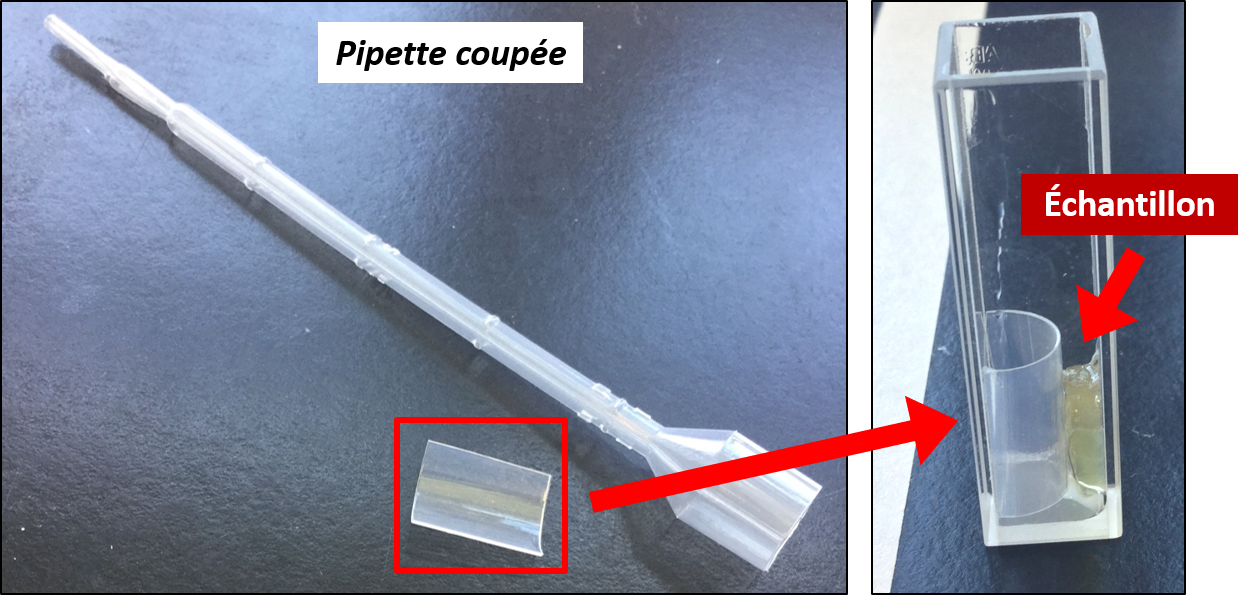
\includegraphics[width=13cm]{pipette.png} \end{center}
        \caption{Exemple de stabilisation de l'échantillon dans la cuvette}
        \begin{footnotesize} Ici, on a une tranche de mésencéphale. On coupe une pipette et on insère le morceau de plastique courbé dans la cuvette. \end{footnotesize}
        \label{fig:pipette}
        \end{figure}
    \item Verser la solution du contenant d'origine dans la cuvette.
    \item Vérifier si l'échantillon est complètement immergé. Si non, ajouter de la solution (même que celle utilisée pour le dernier traitement de la méthode de clarification).
    \item Vérifier qu'il n'y a pas de bulles, de corps étrangers ou autres dans la cuvette.
    \item Mettre le bouchon et sceller avec de la parafilm (voir figure~\ref{fig:parafilm}).
        \begin{figure}[H]
        \centering
        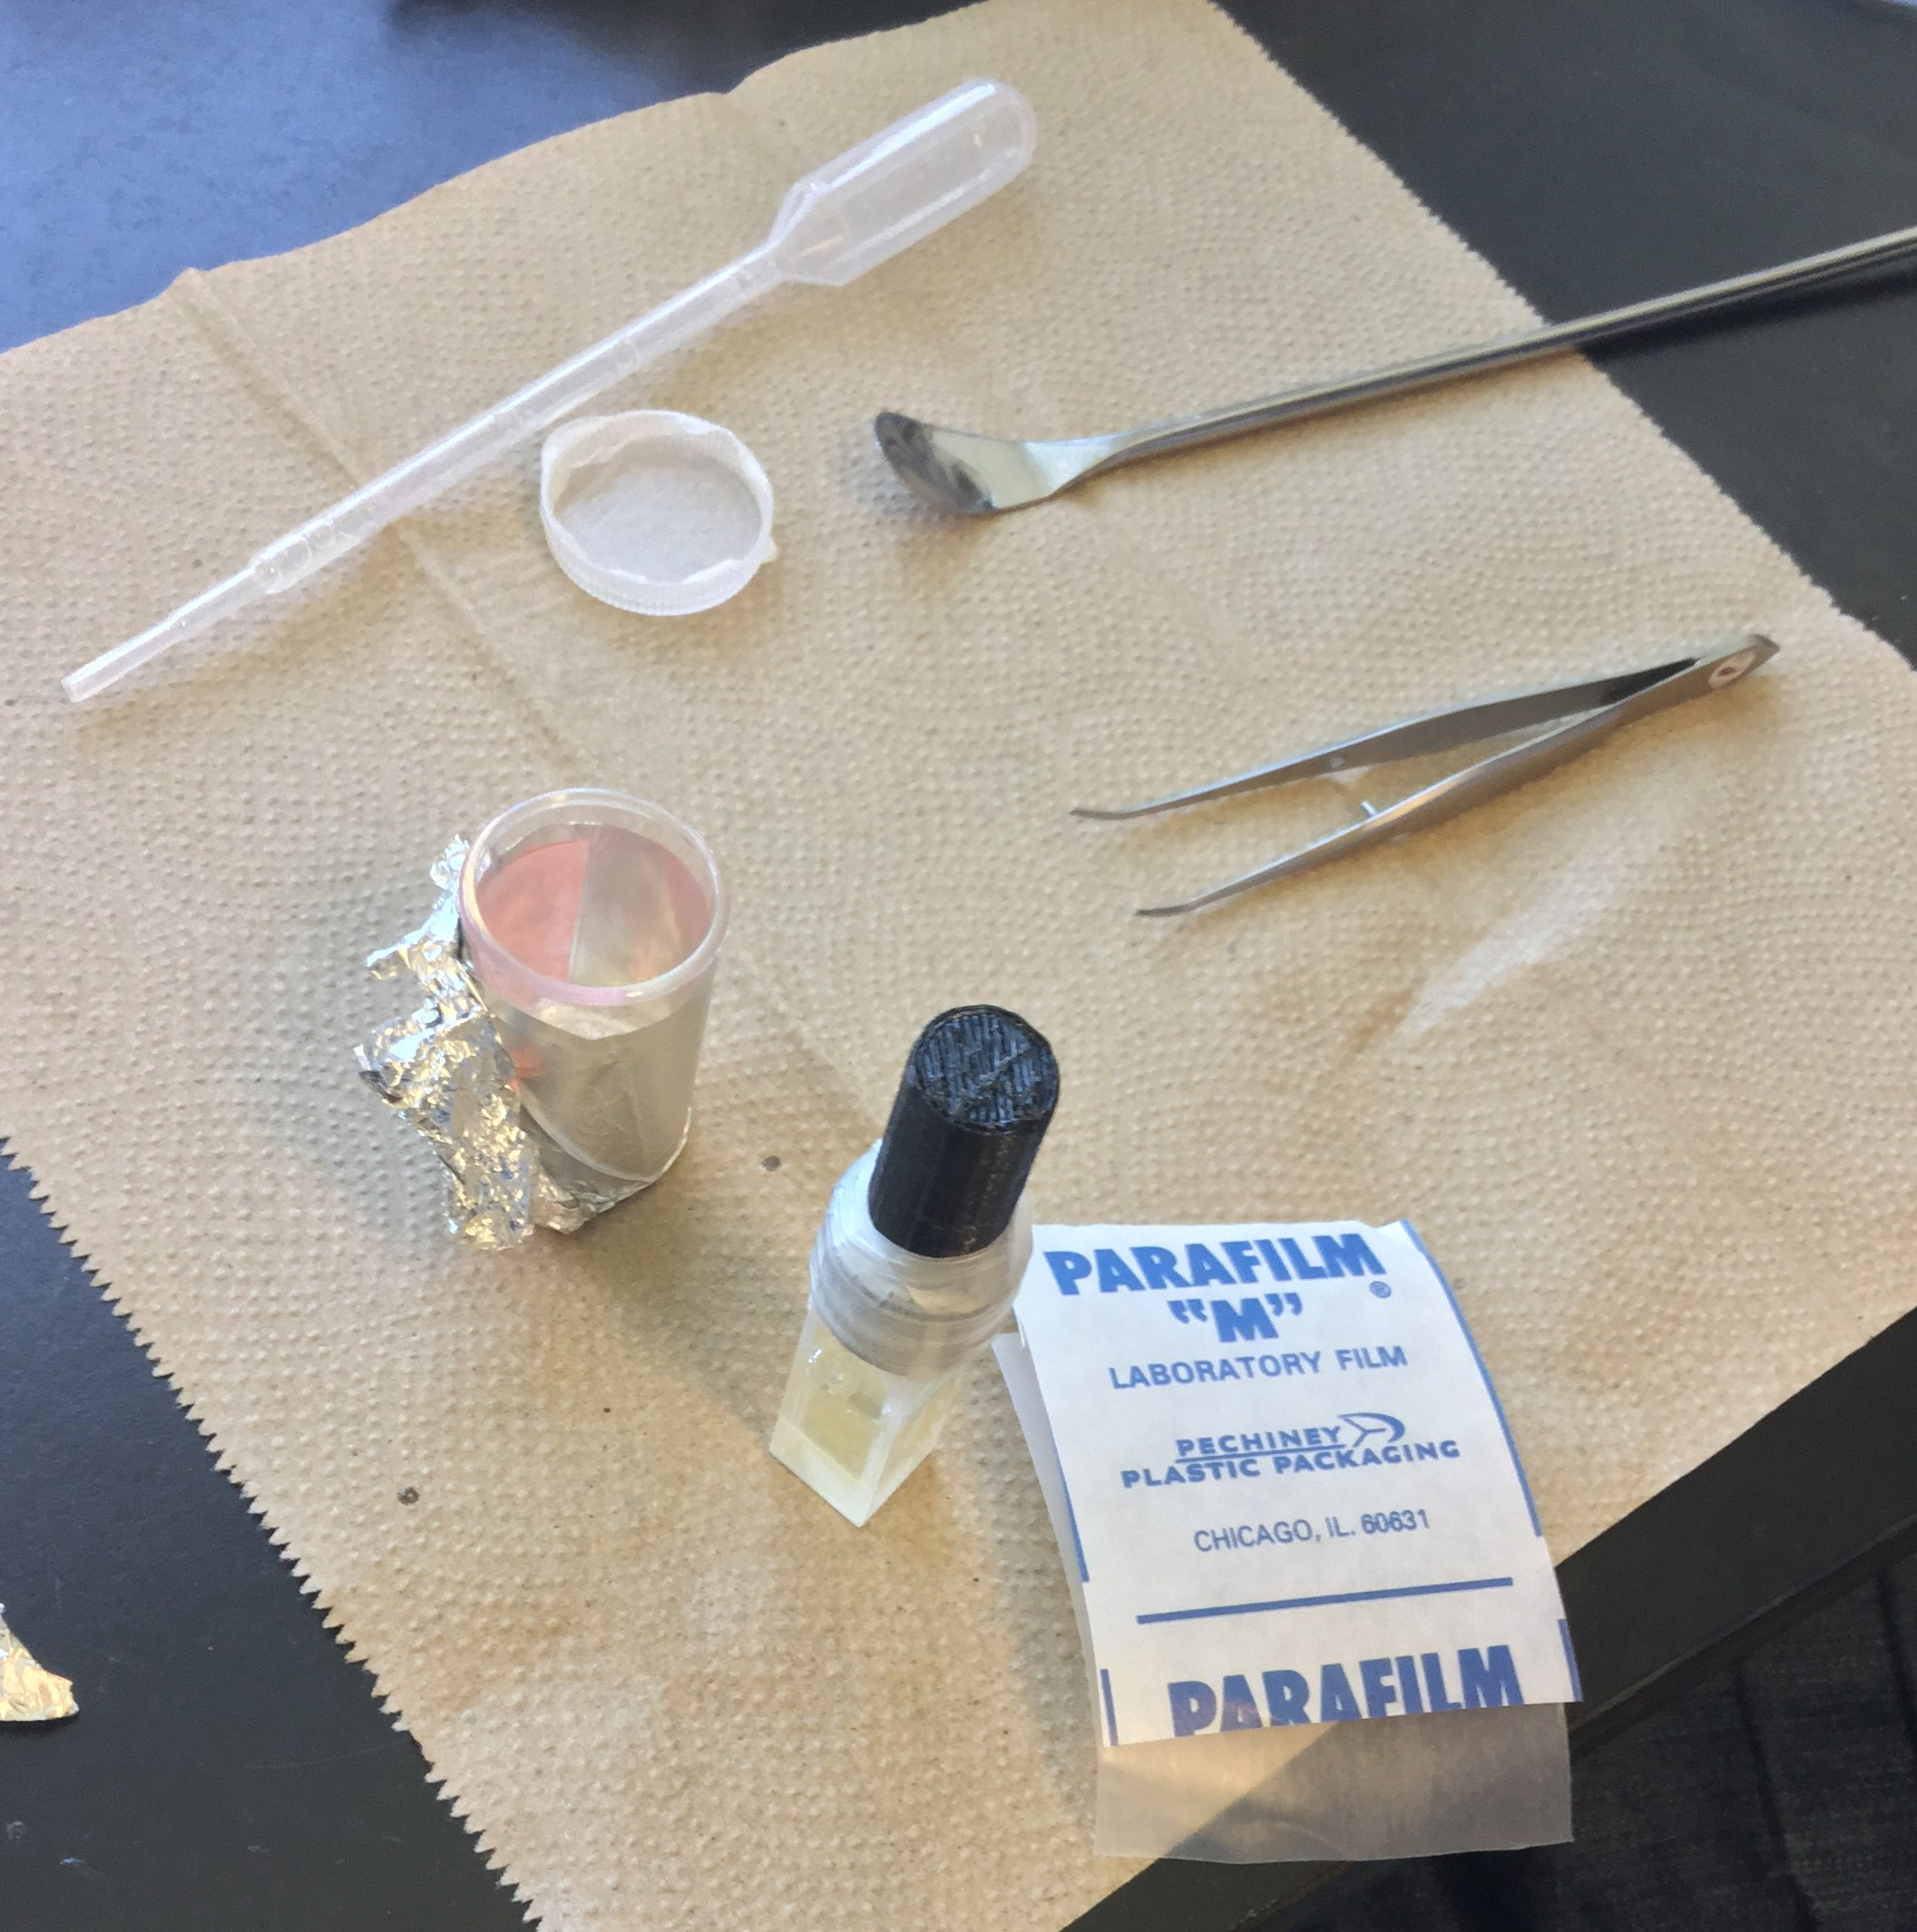
\includegraphics[width=6cm]{parafilm.jpg}
        \caption{Préparation de la cuvette}
        \label{fig:parafilm}
        \end{figure}
\end{enumerate}